\documentclass[12pt,a4paper]{report}
\usepackage[utf8]{inputenc}
\usepackage[T5]{fontenc}
\usepackage[vietnamese]{babel}
\usepackage{amsmath,amssymb}
\usepackage{graphicx}
\usepackage{booktabs}
\usepackage{longtable}
\usepackage{array}
\usepackage{hyperref}
\usepackage{geometry}
\usepackage{fancyhdr}
\usepackage{titlesec}
\usepackage{enumitem}
\usepackage{xcolor}
\usepackage{float}
\usepackage{caption}
\usepackage{subcaption}
\usepackage[expansion=false]{microtype}
\usepackage{parskip}
\usepackage{setspace}
\usepackage{tocloft}
\usepackage[most]{tcolorbox}
\usepackage{tikz}
\usetikzlibrary{arrows.meta, positioning}

% ============ ANALOGY BOX ============
\newtcolorbox{analogybox}[1][]{%
    enhanced, breakable,
    colback=blue!3, colframe=sectioncolor!60,
    coltitle=white, fonttitle=\bfseries\small,
    title={\textit{Ẩn dụ cho người không chuyên}},
    left=8pt, right=8pt, top=6pt, bottom=6pt,
    boxrule=0.6pt, arc=3pt,
    before upper={\small},
    #1
}

% ============ COLORS ============
\definecolor{chaptercolor}{RGB}{0, 51, 102}
\definecolor{sectioncolor}{RGB}{0, 80, 140}
\definecolor{linkblue}{RGB}{0, 90, 160}
\definecolor{titlegray}{RGB}{80, 80, 80}
\definecolor{rulegray}{RGB}{180, 180, 180}
\definecolor{lightbg}{RGB}{245, 247, 250}

% ============ PAGE LAYOUT ============
\geometry{left=2.5cm, right=2cm, top=2.5cm, bottom=2.5cm, headheight=18pt}
\setstretch{1.25}

% ============ HYPERLINKS ============
\hypersetup{
    colorlinks=true,
    linkcolor=chaptercolor,
    citecolor=sectioncolor,
    urlcolor=linkblue
}

% ============ HEADER/FOOTER ============
\pagestyle{fancy}
\fancyhf{}
\fancyhead[L]{\small\color{titlegray}\textit{\leftmark}}
\fancyhead[R]{\small\color{titlegray}\thepage}
\renewcommand{\headrulewidth}{0.3pt}
\renewcommand{\headrule}{\hbox to\headwidth{\color{rulegray}\leaders\hrule height \headrulewidth\hfill}}
\fancyfoot[C]{\small\color{titlegray}\textit{Khảo sát toàn diện sự phát triển của YOLO}}

% ============ CHAPTER TITLE ============
\titleformat{\chapter}[block]
  {\normalfont\huge\bfseries\color{chaptercolor}}
  {\MakeUppercase{\chaptertitlename}\ \thechapter:}
  {15pt}
  {}
\titlespacing*{\chapter}{0pt}{-20pt}{25pt}

% ============ SECTION TITLES ============
\titleformat{\section}
  {\Large\bfseries\color{sectioncolor}}
  {\thesection}{1em}{}
  [\vspace{-4pt}{\color{rulegray}\rule{\textwidth}{0.4pt}}]

\titleformat{\subsection}
  {\large\bfseries\color{chaptercolor!80!black}}
  {\thesubsection}{1em}{}

\titleformat{\subsubsection}
  {\normalsize\bfseries\color{chaptercolor!60!black}\itshape}
  {\thesubsubsection}{1em}{}

% ============ TABLE OF CONTENTS ============
\renewcommand{\cftchapfont}{\bfseries\color{chaptercolor}}
\renewcommand{\cftsecfont}{\color{sectioncolor}}
\renewcommand{\cftchappagefont}{\bfseries\color{chaptercolor}}
\renewcommand{\cftsecpagefont}{\color{sectioncolor}}

% ============ CAPTIONS ============
\captionsetup{
    font={small},
    labelfont={bf,color=sectioncolor},
    textfont={color=titlegray},
    skip=8pt
}

% ============ LIST STYLE ============
\setlist[itemize]{itemsep=2pt, parsep=0pt, topsep=4pt}
\setlist[enumerate]{itemsep=2pt, parsep=0pt, topsep=4pt}

% ============ TITLE PAGE ============
\title{
\vspace{-1cm}
{\color{rulegray}\rule{\textwidth}{1.5pt}}\\[0.8cm]
{\Huge\bfseries\color{chaptercolor} KHẢO SÁT TOÀN DIỆN\\[0.2cm] SỰ PHÁT TRIỂN CỦA YOLO}\\[0.6cm]
{\Large\color{sectioncolor}\textit{Từ YOLOv1 (2015) đến YOLO26 (2026)}}\\[0.3cm]
{\large\color{titlegray} Kiến trúc -- Phương pháp -- Kết quả -- Xu hướng}\\[0.6cm]
{\color{rulegray}\rule{\textwidth}{1.5pt}}
}
\author{
\large\color{chaptercolor}\textbf{Nguyễn Cao Trị}\\[0.3cm]
{\small\color{titlegray} Ngày biên soạn: \today}
}
\date{}

\begin{document}

\maketitle
\thispagestyle{empty}

\newpage
\tableofcontents
\thispagestyle{empty}
\newpage


% ==========================================
% BẮT ĐẦU chuong1_modau
% ==========================================
\chapter{MỞ ĐẦU}

\section{Giới thiệu}

Năm 2015, YOLO (You Only Look Once) tạo bước ngoặt lịch sử khi gom toàn bộ quá trình nhận diện vật thể thành một bước duy nhất (\textbf{one-stage}), giúp AI lần đầu tiên đạt tốc độ thời gian thực (real-time). 

Qua 11 năm (2015–2026) với 14 phiên bản, YOLO đã "dân chủ hóa" thị giác máy tính, đưa công nghệ từ phòng thí nghiệm ứng dụng thẳng vào y tế, xe tự hành và các thiết bị Edge AI siêu nhỏ.

\section{Phạm vi báo cáo}

Báo cáo này là bức tranh toàn cảnh về sự tiến hóa của YOLO, tập trung vào ba trọng tâm:

\begin{itemize}
    \item \textbf{Kiến trúc dòng chính:} Đánh giá đột phá kỹ thuật qua từng thời kỳ: khai mở (v1--v4), bùng nổ (v5--v8), nâng cấp Attention/NMS-free (v9--v12) và sự tinh giản Edge-First (YOLO26).
    \item \textbf{Biến thể nổi bật:} Khảo sát các nhánh rẽ công nghiệp có ảnh hưởng lớn (YOLOX, PP-YOLOE, YOLO-NAS).
    \item \textbf{So sánh đa chiều:} Phân tích sự đánh đổi (trade-off) giữa Độ chính xác (mAP) và Tốc độ (FPS/MACs) nhằm đưa ra định hướng lựa chọn mô hình thực tiễn.
\end{itemize}

% KẾT THÚC chuong1_modau
% ==========================================


% ==========================================
% BẮT ĐẦU chuong2_nentang
% ==========================================
\chapter{NỀN TẢNG LÝ THUYẾT}
\section{Kiến trúc chung (Pipeline)}
\begin{figure}[H]
\centering
\begin{tikzpicture}[
    node distance=0.8cm,
    box/.style={rectangle, draw=sectioncolor, fill=blue!5, thick, minimum width=10cm, minimum height=1.3cm, align=center, rounded corners=4pt},
    arrow/.style={-{Stealth[scale=1.2]}, thick, color=sectioncolor}
]

\node[box, fill=gray!10, draw=gray, dashed] (input) {\textbf{Ảnh đầu vào} (Input Image)};

\node[box, below=of input] (backbone) {\begin{tabular}{c}\textbf{\textcolor{chaptercolor}{Backbone (Xương sống)}}\\ \small\textcolor{titlegray}{"Đôi mắt": Trích xuất đặc trưng hình ảnh (Darknet, CSPDarknet)}\end{tabular}};

\node[box, below=of backbone] (neck) {\begin{tabular}{c}\textbf{\textcolor{chaptercolor}{Neck (Cổ)}}\\ \small\textcolor{titlegray}{"Bộ trộn": Kết hợp đặc trưng lớn nhỏ để nhận diện đa kích thước (FPN, PANet)}\end{tabular}};

\node[box, below=of neck] (head) {\begin{tabular}{c}\textbf{\textcolor{chaptercolor}{Head (Đầu)}}\\ \small\textcolor{titlegray}{"Bộ não": Xuất ra tọa độ khung bao (BBox) và nhãn (Class)}\end{tabular}};

\node[box, fill=gray!10, draw=gray, dashed, below=of head] (output) {\textbf{Kết quả} (Bounding Boxes \& Classes)};

\draw[arrow] (input) -- (backbone);
\draw[arrow] (backbone) -- (neck);
\draw[arrow] (neck) -- (head);
\draw[arrow] (head) -- (output);
\end{tikzpicture}
\caption{Pipeline 3 thành phần tiêu chuẩn của mô hình YOLO}
\end{figure}

\section{Khái niệm \& Thước đo cốt lõi}
\begin{itemize}
    \item \textbf{mAP (mean Average Precision):} Thang đo độ chính xác. Tiêu chuẩn vàng hiện nay là \textbf{mAP@50:95} đo trên tập dữ liệu \textbf{MS COCO}.
    \item \textbf{Anchor Boxes (Khung neo):} Khung đoán mẫu. Các đời cũ (v2--v7) bị lệ thuộc vào khung này (Anchor-based). Từ v8 trở đi đã bỏ hẳn để linh hoạt hơn (Anchor-free).
    \item \textbf{NMS (Non-Maximum Suppression):} Bộ lọc xóa các dự đoán trùng lặp. Đã bị khai tử từ YOLOv10 (NMS-free) để tối đa hóa tốc độ.
\end{itemize}

% KẾT THÚC chuong2_nentang
% ==========================================


% ==========================================
% BẮT ĐẦU chuong3_yolov1v4
% ==========================================
\chapter[Thế Hệ Đầu: YOLOv1 - YOLOv4]{\protect\newline Thế Hệ Đầu: YOLOv1 - YOLOv4}

%% ========== YOLOv1 ==========
\section{YOLOv1 (2015) --- Khởi nguồn}
\textbf{Paper:} ``You Only Look Once: Unified, Real-Time Object Detection'' (CVPR 2016) \cite{yolov1}\\
\textbf{Tác giả:} Joseph Redmon, Santosh Divvala, Ross Girshick, Ali Farhadi

\begin{figure}[H]
\centering
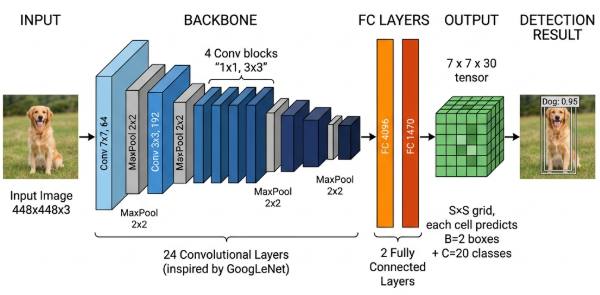
\includegraphics[width=\textwidth]{yolov1_arch.png}
\caption{Kiến trúc YOLOv1: 24 Conv layers + 2 FC layers. Input $448 \times 448$ $\rightarrow$ Output tensor $7 \times 7 \times 30$ (dựa theo Figure 3, Redmon et al. 2016 \cite{yolov1}).}
\end{figure}

\subsection{Ý tưởng cốt lõi}
Coi object detection là \textbf{bài toán hồi quy duy nhất}: từ pixel ảnh $\rightarrow$ bounding boxes + class probabilities, chỉ qua \textbf{một lần forward pass}. Chia ảnh thành lưới $S \times S$ ($S=7$), mỗi ô dự đoán $B=2$ boxes và $C=20$ classes \cite{yolov1}.

\subsection{Kiến trúc}
24 lớp convolutional + 2 lớp fully connected. Cảm hứng từ GoogLeNet. Output: tensor $7 \times 7 \times 30$. Fast YOLO: 9 conv layers.

\subsection{Nhận xét}

\textbf{Có gì mới?}
\begin{itemize}
    \item Là mô hình \textbf{one-stage đầu tiên} trong lịch sử: gom detection thành một phép hồi quy duy nhất, bỏ qua hoàn toàn bước đề xuất vùng (region proposal) vốn rất chậm của R-CNN.
    \item Đạt \textbf{45 FPS} (phiên bản Fast YOLO: 155 FPS) --- nhanh gấp \textbf{90$\times$} so với Fast R-CNN (0.5 FPS), lần đầu tiên cho phép chạy detection trên video thời gian thực.
    \item Nhìn toàn bộ ảnh cùng lúc nên hiểu ngữ cảnh tốt hơn, giảm mạnh lỗi nhận nhầm nền thành vật thể (false positive background giảm hơn 50\% so với R-CNN).
\end{itemize}

\textbf{Hạn chế:}
\begin{itemize}
    \item Lưới $7\times7$ quá thô $\rightarrow$ mỗi ô chỉ dự đoán được 2 box và 1 class duy nhất. Khi nhiều vật nhỏ nằm cùng một ô (ví dụ: đàn chim đậu sát nhau), model chỉ phát hiện được 1 con và bỏ sót phần còn lại.
    \item Độ chính xác định vị (localization) kém, đặc biệt với vật thể có tỉ lệ khung hình bất thường (quá dài hoặc quá rộng).
\end{itemize}

\textbf{Ví dụ:} Hãy hình dung bạn cần tìm tất cả các chú chó trong một bức ảnh. Mô hình cũ (R-CNN) dùng kính lúp soi từng góc ảnh --- chính xác nhưng mất cả phút. YOLOv1 thì kẻ ảnh thành bàn cờ $7\times7$, lùi lại một bước nhìn tổng thể và đánh dấu ngay ô nào chứa chó --- chỉ trong $\frac{1}{45}$ giây. Đổi lại, nếu hai chú chó đứng quá gần nhau trong cùng một ô, YOLOv1 chỉ ``thấy'' được một con.

%% ========== YOLOv2 ==========
\section{YOLOv2 / YOLO9000 (2016) --- Better, Faster, Stronger}
\textbf{Paper:} ``YOLO9000: Better, Faster, Stronger'' (CVPR 2017) \cite{yolov2}\\
\textbf{Tác giả:} Joseph Redmon, Ali Farhadi

\subsection{Ý tưởng cốt lõi}
Vá triệt để các lỗi của v1 bằng 7 kỹ thuật cải tiến tích lũy, đồng thời mở rộng khả năng nhận diện lên hơn 9000 loại vật thể thông qua cơ chế WordTree.

\subsection{Kiến trúc}
Backbone mới \textbf{Darknet-19} (19 conv + 5 maxpool), chỉ tốn 5.58B FLOPs (VGG-16: 30.69B). Lần đầu giới thiệu \textbf{Anchor Boxes} --- 5 khung neo được tìm tự động bằng k-means trên dataset.

\subsection{Nhận xét}

\textbf{Có gì mới?}
\begin{itemize}
    \item Thêm \textbf{Batch Normalization} vào mọi conv layer $\rightarrow$ bỏ Dropout, tăng +2\% mAP.
    \item Giới thiệu \textbf{Anchor Boxes}: thay vì đoán tọa độ box từ con số 0 (như v1), model chỉ cần ``tinh chỉnh'' các khung mẫu có sẵn $\rightarrow$ recall tăng +7\%.
    \item Huấn luyện trên \textbf{nhiều kích thước ảnh} (multi-scale: 320--608) $\rightarrow$ model linh hoạt hơn.
    \item Tổng cộng: mAP nhảy từ 63.4\% lên \textbf{76.8\%} (+13.4\%) trên VOC 2007.
\end{itemize}

\textbf{Hạn chế:}
\begin{itemize}
    \item Anchor boxes cố định theo dataset $\rightarrow$ chuyển sang dataset mới phải chạy lại k-means.
    \item Vẫn chỉ dự đoán ở \textbf{1 scale duy nhất} ($13\times13$), nên vật nhỏ vẫn bị bỏ sót.
\end{itemize}

\textbf{Ví dụ:} Nếu YOLOv1 giống ``vẽ tay tự do'' khung bao quanh vật (dễ méo, dễ sai kích thước), thì YOLOv2 giống ``chọn từ 5 khuôn mẫu có sẵn'' rồi chỉnh nhẹ --- nhanh hơn và chuẩn hơn rất nhiều.

%% ========== YOLOv3 ==========
\section{YOLOv3 (2018) --- Multi-Scale Detection}
\textbf{Paper:} ``YOLOv3: An Incremental Improvement'' (Tech Report) \cite{yolov3}\\
\textbf{Tác giả:} Joseph Redmon, Ali Farhadi \textit{(paper cuối cùng của Redmon trước khi dừng nghiên cứu CV vì lo ngại đạo đức)}

\subsection{Ý tưởng cốt lõi}
Dự đoán vật thể ở \textbf{3 kích thước khác nhau} (3 scales) theo phong cách Feature Pyramid Network (FPN), vá dứt điểm lỗi ``mù vật nhỏ'' của v1 và v2.

\subsection{Kiến trúc}
Backbone mới \textbf{Darknet-53} (53 conv layers + residual connections). Chính xác ngang ResNet-152 nhưng \textbf{nhanh gấp 2$\times$} (78 vs 37 FPS). Head dự đoán ở 3 feature maps: $13\times13$, $26\times26$, $52\times52$ với 3 anchors/scale = 9 anchors tổng.

\subsection{Nhận xét}

\textbf{Có gì mới?}
\begin{itemize}
    \item \textbf{3 scales} detection: feature map $52\times52$ chuyên bắt vật nhỏ, $13\times13$ chuyên bắt vật lớn $\rightarrow$ bao phủ mọi kích thước.
    \item Thay \textbf{Softmax} bằng \textbf{Sigmoid} cho classification $\rightarrow$ hỗ trợ multi-label (một vật có thể vừa là ``người'' vừa là ``phụ nữ'').
    \item Residual connections giúp train mạng sâu 53 layers mà không bị vanishing gradient.
    \item mAP@50 đạt \textbf{57.9\%} trên COCO, ngang RetinaNet nhưng nhanh gấp \textbf{3.8$\times$}.
\end{itemize}

\textbf{Hạn chế:}
\begin{itemize}
    \item mAP@50:95 chỉ đạt 33.0\% $\rightarrow$ khi yêu cầu IoU cao, khả năng localization vẫn kém.
    \item Vẫn phụ thuộc NMS để lọc kết quả trùng lặp.
\end{itemize}

\textbf{Ví dụ:} YOLOv2 giống camera chỉ có 1 ống kính zoom cố định --- chụp phong cảnh đẹp nhưng côn trùng nhỏ thì mờ. YOLOv3 giống camera có \textbf{3 ống kính} (wide, normal, tele): ống wide bắt cả sân, ống tele bắt rõ con ong trên cành hoa.

%% ========== YOLOv4 ==========
\section{YOLOv4 (2020) --- Tập đại thành}
\textbf{Paper:} ``YOLOv4: Optimal Speed and Accuracy of Object Detection'' \cite{yolov4}\\
\textbf{Tác giả:} Alexey Bochkovskiy, Chien-Yao Wang, Hong-Yuan Mark Liao

\begin{figure}[H]
\centering
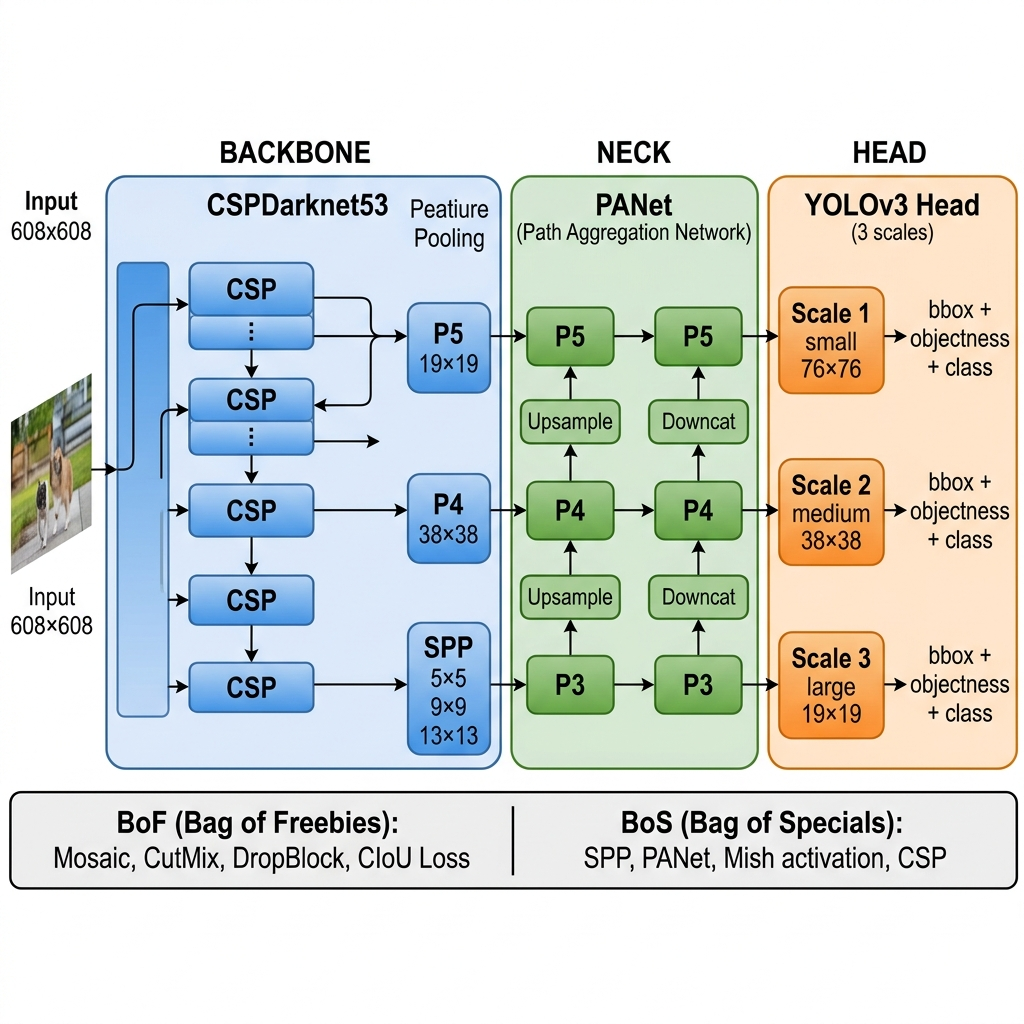
\includegraphics[width=\textwidth]{yolov4_arch.png}
\caption{Kiến trúc YOLOv4: CSPDarknet53 (Backbone) + SPP + PANet (Neck) + YOLOv3 Head \cite{yolov4}.}
\end{figure}

\subsection{Ý tưởng cốt lõi}
Hệ thống hóa hàng trăm kỹ thuật tăng cường thành 2 nhóm: \textbf{Bag of Freebies} (miễn phí khi inference) và \textbf{Bag of Specials} (tốn thêm chút inference), rồi tìm tổ hợp tối ưu trên single GPU.

\subsection{Kiến trúc}
\textbf{CSPDarknet53} chia features thành 2 phần xử lý song song rồi gộp lại $\rightarrow$ giảm \textbf{20\% computation}. Neck: \textbf{SPP} (tăng receptive field) + \textbf{PANet} (cải thiện localization).

\subsection{Nhận xét}

\textbf{Có gì mới?}
\begin{itemize}
    \item \textbf{Mosaic Augmentation}: Ghép 4 ảnh thành 1 $\rightarrow$ model học nhiều ngữ cảnh hơn, giảm batch size (train trên 1 GPU thay vì 8 GPU).
    \item \textbf{CIoU Loss}: Xét cùng lúc overlap, khoảng cách tâm, và tỉ lệ khung $\rightarrow$ localization chính xác hơn hẳn.
    \item Đạt \textbf{43.5\% mAP} trên COCO ở 65 FPS (V100) --- nhảy vọt \textbf{+10.5\%} so với v3, bước nhảy lớn nhất lịch sử YOLO.
    \item Là YOLO đầu tiên có thể \textbf{train trên single GPU} mà vẫn đạt SOTA.
\end{itemize}

\textbf{Hạn chế:}
\begin{itemize}
    \item Vẫn viết bằng Darknet (C) $\rightarrow$ khó tích hợp vào pipeline Python/PyTorch hiện đại.
    \item Kiến trúc phức tạp, nhiều ``kỹ xảo'' $\rightarrow$ khó tùy biến cho người mới.
\end{itemize}

\textbf{Ví dụ:} Nếu v3 giống chiếc xe đua tốt nhưng chỉ chạy trên đường thẳng, thì v4 giống xe được ``độ'' toàn diện --- thay lốp mới (CIoU), gắn turbo (Mosaic), nâng cấp hộp số (CSPNet) --- để chạy nhanh hơn trên \textbf{mọi địa hình}, kể cả đường xấu (dataset nhỏ, 1 GPU).

% KẾT THÚC chuong3_yolov1v4
% ==========================================


% ==========================================
% BẮT ĐẦU chuong4_yolov5v8
% ==========================================
\chapter{THẾ HỆ GIỮA: YOLOv5 -- YOLOv8 (2020--2023)}

%% ========== YOLOv5 ==========
\section{YOLOv5 (2020) --- Dân chủ hóa YOLO}
\textbf{Tác giả:} Glenn Jocher / Ultralytics \hfill \textbf{Framework:} PyTorch \hfill \textit{Không có paper}

\subsection{Ý tưởng cốt lõi}
Chuyển YOLO từ framework Darknet (C) sang \textbf{PyTorch}, biến YOLO từ công cụ hàn lâm thành sản phẩm công nghiệp mà ai cũng dùng được chỉ với 3 dòng Python:
\begin{verbatim}
    from ultralytics import YOLO
    model = YOLO('yolov5s.pt')
    results = model('anh.jpg')
\end{verbatim}

\subsection{Kiến trúc}
Backbone: \textbf{CSPDarknet53 (modified)} với \textbf{C3 module}. Neck: PANet + \textbf{SPPF} (3 MaxPool nối tiếp thay vì song song, nhanh gấp 2$\times$). Head: Anchor-based, 3 scales, có \textbf{AutoAnchor} tự tìm anchor tối ưu. Ra mắt \textbf{5 kích cỡ model}: Nano, Small, Medium, Large, XLarge.

\subsection{Nhận xét}

\textbf{Có gì mới?}
\begin{itemize}
    \item \textbf{Dễ dùng bậc nhất}: \texttt{pip install ultralytics}, export 10+ định dạng (ONNX, TensorRT, CoreML...) $\rightarrow$ trở thành YOLO phổ biến nhất mọi thời đại.
    \item \textbf{5 sizes} phủ từ IoT (Nano: 1.9M params) đến server (XLarge: 86.7M params).
    \item \textbf{SPPF} tăng tốc SPP gấp 2$\times$ mà kết quả tương đương.
    \item mAP cao nhất đạt \textbf{50.7\%} (v5x) trên COCO.
\end{itemize}

\textbf{Hạn chế:}
\begin{itemize}
    \item Không có paper $\rightarrow$ không được peer-reviewed, cộng đồng học thuật hoài nghi.
    \item Kiến trúc gần giống v4, chưa có đột phá kỹ thuật thực sự.
    \item Vẫn dùng \textbf{Anchor-based} --- cần tune anchor cho từng dataset.
\end{itemize}

\textbf{Ví dụ:} YOLOv4 giống siêu xe cần thợ chuyên nghiệp để lái (compile C, config file phức tạp). YOLOv5 giống \textbf{xe tự lái Tesla} --- ai cũng lên xe bấm nút là chạy, không cần biết cơ khí.

%% ========== YOLOv6 ==========
\section{YOLOv6 (2022) --- Industrial Deployment}
\textbf{Paper:} ``YOLOv6: A Single-Stage Object Detection Framework for Industrial Applications''\\
\textbf{Tác giả:} Meituan Vision AI (dịch vụ giao đồ ăn lớn nhất Trung Quốc)

\subsection{Ý tưởng cốt lõi}
Dùng kỹ thuật \textbf{Re-parameterization}: kiến trúc \textbf{khác nhau giữa training và inference}. Khi train dùng multi-branch (học phong phú), khi deploy gộp thành 1 Conv duy nhất (chạy nhanh). Tối ưu đặc biệt cho \textbf{quantization INT8} trên GPU server.

\subsection{Kiến trúc}
Backbone: \textbf{EfficientRep} (RepVGG blocks). Neck: \textbf{Rep-PAN}. Head: \textbf{Efficient Decoupled Head} (tách classification/regression). Chuyển sang \textbf{Anchor-free} (dự đoán 4 khoảng cách từ tâm, kiểu FCOS).

\subsection{Nhận xét}

\textbf{Có gì mới?}
\begin{itemize}
    \item \textbf{Re-parameterization}: Train với 3 branch song song, deploy gộp thành 1 branch $\rightarrow$ accuracy cao + inference nhanh.
    \item \textbf{Quantization pipeline} (PTQ $\rightarrow$ QAT): INT8 chỉ mất \textbf{0.2\% mAP} nhưng tăng \textbf{75\% FPS}.
    \item Vượt v5 ở \textbf{mọi scale}, đặc biệt Nano đạt \textbf{1187 FPS} (v5n: 602 FPS).
\end{itemize}

\textbf{Hạn chế:}
\begin{itemize}
    \item Ecosystem nhỏ hơn v5 rất nhiều, ít tài liệu hướng dẫn.
    \item Chủ yếu tối ưu cho GPU server (T4), chưa phổ biến trên edge devices.
\end{itemize}

\textbf{Ví dụ:} Hãy hình dung ôn thi: khi ôn (training), bạn đọc 5 cuốn sách, ghi chú, làm bài tập (multi-branch). Khi vào phòng thi (inference), bạn chỉ cần \textbf{1 tờ tóm tắt} chứa tinh hoa từ 5 cuốn --- đó là Re-parameterization.

%% ========== YOLOv7 ==========
\section{YOLOv7 (2022) --- SOTA Accuracy}
\textbf{Paper:} ``YOLOv7: Trainable Bag-of-Freebies Sets New State-of-the-Art'' (CVPR 2023)\\
\textbf{Tác giả:} Chien-Yao Wang, Alexey Bochkovskiy, Hong-Yuan Mark Liao

\subsection{Ý tưởng cốt lõi}
Mở rộng ELAN thành \textbf{E-ELAN} (tăng số nhánh song song mà không phá gradient path gốc), kết hợp với hệ thống \textbf{Lead Head + Auxiliary Head} --- head phụ chỉ dùng khi training để tạo thêm tín hiệu học, bỏ khi inference.

\subsection{Kiến trúc}
Backbone: \textbf{E-ELAN} (Extended Efficient Layer Aggregation). Dùng \textbf{RepConvN} (bỏ identity branch để tránh xung đột gradient khi có residual). Head: Coarse-to-Fine label assignment với Lead + Auxiliary heads.

\subsection{Nhận xét}

\textbf{Có gì mới?}
\begin{itemize}
    \item \textbf{E-ELAN}: Tăng cardinality (số nhánh) + shuffle + merge $\rightarrow$ features phong phú hơn (+0.7\% mAP).
    \item \textbf{Auxiliary Head}: Head phụ gán nhãn lỏng hơn $\rightarrow$ tạo nhiều training signal, \textbf{zero inference cost}.
    \item YOLOv7 (36.9M params) đạt \textbf{51.4\% mAP} ở 161 FPS --- ít params nhất và nhanh nhất so với v5-L, YOLOX-L, PPYOLOE-L.
    \item YOLOv7-E6E đạt \textbf{56.8\% mAP} --- vượt cả Transformer-based (SWIN-L: 53.9\%).
\end{itemize}

\textbf{Hạn chế:}
\begin{itemize}
    \item Kiến trúc phức tạp (E-ELAN, RepConvN, dual head) $\rightarrow$ khó implement và debug.
    \item Ecosystem không mạnh bằng Ultralytics (v5/v8), ít người dùng ngoài nghiên cứu.
\end{itemize}

\textbf{Ví dụ:} Auxiliary Head giống \textbf{trợ giảng} trong lớp học: giáo viên chính (Lead Head) chấm điểm nghiêm khắc, trợ giảng cho điểm nhẹ nhàng hơn $\rightarrow$ sinh viên nhận nhiều feedback $\rightarrow$ học tốt hơn. Khi thi thật (inference), chỉ có giáo viên chính chấm.

%% ========== YOLOv8 ==========
\section{YOLOv8 (2023) --- Đa năng nhất}
\textbf{Tác giả:} Ultralytics \hfill \textit{Không có paper}

\subsection{Ý tưởng cốt lõi}
Bỏ hoàn toàn Anchor Boxes (chuyển sang \textbf{Anchor-Free}), tách detection head thành 2 nhánh riêng biệt (\textbf{Decoupled Head}), và mở rộng thành \textbf{framework đa tác vụ}: Detection, Segmentation, Classification, Pose Estimation, OBB, Tracking --- tất cả trong cùng 1 API.

\subsection{Kiến trúc}
Backbone: CSPDarknet với \textbf{C2f module} (concat output của TẤT CẢ bottlenecks thay vì chỉ output cuối $\rightarrow$ gradient flow phong phú hơn). Head: Anchor-free, Decoupled, dùng \textbf{DFL (Distribution Focal Loss)} --- dự đoán phân phối xác suất trên 16 bins thay vì 1 giá trị duy nhất cho mỗi tọa độ.

\subsection{Nhận xét}

\textbf{Có gì mới?}
\begin{itemize}
    \item \textbf{Anchor-Free}: Dự đoán center point + 4 khoảng cách, không cần tune anchor nữa.
    \item \textbf{DFL}: Mô hình hóa ``sự không chắc chắn'' khi định vị cạnh box $\rightarrow$ localization chính xác hơn.
    \item \textbf{6 tác vụ} trong 1 framework: Detection, Segmentation, Classification, Pose, OBB, Tracking.
    \item v8n đạt \textbf{37.3\% mAP} (+9.3\% so với v5n), v8x đạt \textbf{53.9\%}.
\end{itemize}

\textbf{Hạn chế:}
\begin{itemize}
    \item v8-X (53.9\%) \textbf{thua} v7-E6E (56.8\%) về mAP thuần túy.
    \item Không có paper chính thức $\rightarrow$ không rõ chi tiết thí nghiệm.
\end{itemize}

\textbf{Ví dụ:} Nếu cần \textbf{accuracy tối đa} $\rightarrow$ chọn v7. Nếu cần \textbf{đa năng + dễ dùng} $\rightarrow$ chọn v8. DFL giống khi nói ``cạnh trái cách tâm khoảng 25px'' --- thay vì nói ``đúng 25px'' (1 số), DFL nói ``70\% khả năng ở 25px, 20\% ở 26px, 10\% ở 24px'' $\rightarrow$ phản ánh sự không chắc chắn, chính xác hơn.

% KẾT THÚC chuong4_yolov5v8
% ==========================================


% ==========================================
% BẮT ĐẦU chuong5_yolov9v12
% ==========================================
\chapter{THẾ HỆ MỚI: YOLOv9 -- YOLOv12 (2024--2025)}

%% ========== YOLOv9 ==========
\section{YOLOv9 (2024) --- Chống mất thông tin}
\textbf{Paper:} ``YOLOv9: Learning What You Want to Learn Using Programmable Gradient Information''\\
\textbf{Tác giả:} Chien-Yao Wang, I-Hau Yeh, Hong-Yuan Mark Liao

\subsection{Ý tưởng cốt lõi}
Giải quyết vấn đề \textbf{Information Bottleneck}: khi data đi qua nhiều layers, thông tin bị mất dần (giống trò ``truyền tin'' qua 20 người). Giải pháp: thêm một \textbf{nhánh phụ có khả năng khôi phục thông tin gốc} (PGI) chạy song song khi training, bỏ khi inference.

\subsection{Kiến trúc}
Backbone: \textbf{GELAN} (Generalized ELAN) --- cho phép dùng bất kỳ loại block nào bên trong (Conv, Bottleneck, Transformer...). Training: thêm \textbf{PGI} (Programmable Gradient Information) với auxiliary reversible branch để giữ full information $\rightarrow$ gradient đáng tin cậy.

\subsection{Nhận xét}

\textbf{Có gì mới?}
\begin{itemize}
    \item \textbf{PGI}: Nhánh phụ reversible giữ toàn bộ thông tin input $\rightarrow$ gradient luôn chính xác, đặc biệt hiệu quả cho lightweight models (+2.5\% AP).
    \item \textbf{GELAN}: Dây chuyền ``universal'' --- lắp block gì vào cũng chạy, linh hoạt hơn ELAN cũ.
    \item v9 luôn \textbf{ít params hơn} v8 mà accuracy cao hơn ở mọi scale: v9-E đạt \textbf{55.6\%} (v8-X: 53.9\%, +1.7\%).
\end{itemize}

\textbf{Hạn chế:}
\begin{itemize}
    \item PGI chỉ có tác dụng khi training, nên lợi ích phụ thuộc vào chất lượng auxiliary branch.
    \item Ecosystem nhỏ, chưa được tích hợp rộng rãi vào Ultralytics.
\end{itemize}

\textbf{Ví dụ:} PGI giống hệ thống \textbf{SMS đối chiếu}: main branch là ``truyền miệng'' qua 20 người (mất thông tin dần), PGI thêm 1 kênh SMS song song --- mỗi người đều nhận SMS gốc để đối chiếu và sửa sai kịp thời.

%% ========== YOLOv10 ==========
\section{YOLOv10 (2024) --- NMS-Free}
\textbf{Paper:} ``YOLOv10: Real-Time End-to-End Object Detection''\\
\textbf{Tác giả:} Ao Wang et al. (Tsinghua University)

\subsection{Ý tưởng cốt lõi}
Loại bỏ hoàn toàn \textbf{NMS} (Non-Maximum Suppression) bằng hệ thống \textbf{Consistent Dual Assignments}: dùng 2 head --- one-to-many (train tốt) và one-to-one (deploy không cần NMS). Khi inference chỉ dùng head one-to-one.

\subsection{Kiến trúc}
Kế thừa v8 nhưng thêm 5 kỹ thuật efficiency: lightweight cls head (depthwise separable), decoupled downsample, rank-guided block, large-kernel conv ($7\times7$), và PSA (partial self-attention, chỉ 50\% channels qua attention).

\subsection{Nhận xét}

\textbf{Có gì mới?}
\begin{itemize}
    \item \textbf{NMS-Free}: Không cần bước hậu xử lý $\rightarrow$ latency ổn định, không phụ thuộc số vật trong ảnh.
    \item v10-S đạt \textbf{46.3\% mAP} ở latency 2.49ms --- nhanh gấp \textbf{2$\times$} so với v8-S+NMS (4.70ms).
    \item v10-X chỉ cần \textbf{29.5M params} (v8-X: 68.2M) --- ít hơn 2.3$\times$.
\end{itemize}

\textbf{Hạn chế:}
\begin{itemize}
    \item v10-X (54.4\%) \textbf{thua} v9-E (55.6\%) về mAP --- đổi accuracy lấy efficiency.
    \item Dual head làm tăng complexity khi training.
\end{itemize}

\textbf{Ví dụ:} NMS giống kiểm tra chất lượng cuối dây chuyền sản xuất --- phải dừng lại soi từng sản phẩm, loại phế phẩm. v10 thiết kế dây chuyền ``zero defect'' --- sản phẩm ra là đạt chuẩn ngay, không cần kiểm tra cuối.

%% ========== YOLO11 ==========
\section{YOLO11 (2024) --- Nâng cấp toàn diện}
\textbf{Tác giả:} Ultralytics \hfill \textit{Không có paper} \hfill \textit{Lưu ý: bỏ ``v'' --- YOLO11 thay vì YOLOv11}

\subsection{Ý tưởng cốt lõi}
Nâng cấp C2f (v8) thành \textbf{C3K2} (dùng 2 kernel sizes: $3\times3$ và $5\times5$ trong cùng 1 block) và thêm \textbf{C2PSA} (spatial attention) để model tự học ``vùng nào quan trọng'' trong ảnh.

\subsection{Kiến trúc}
Backbone: CSPDarknet với \textbf{C3K2} (multi-scale feature extraction trong cùng 1 block). Neck: thêm \textbf{C2PSA} (Cross Stage Partial Spatial Attention) --- attention map highlight vùng có vật thể, suppress background.

\subsection{Nhận xét}

\textbf{Có gì mới?}
\begin{itemize}
    \item \textbf{C3K2}: 2 kernel ($3\times3$ + $5\times5$) vừa thấy chi tiết nhỏ vừa thấy bối cảnh rộng --- phong phú hơn C2f (chỉ $3\times3$).
    \item \textbf{C2PSA}: Tập trung vào vùng quan trọng như mắt người, lướt nhanh qua background.
    \item Cải thiện ở \textbf{mọi scale}: 11n đạt \textbf{39.5\%} (+2.2\% so với v8n), 11x đạt \textbf{54.7\%} (+0.8\%).
\end{itemize}

\textbf{Hạn chế:}
\begin{itemize}
    \item Cải tiến incremental, chưa có đột phá kiến trúc lớn.
    \item Không có paper chính thức.
\end{itemize}

\textbf{Ví dụ:} C2f (v8) giống nhìn qua 1 ống kính cố định --- mọi pixel xử lý ngang nhau. C3K2 giống nhìn qua \textbf{2 ống kính zoom khác nhau} cùng lúc, còn C2PSA giống \textbf{mắt người} --- tự động tập trung vào vật thể, lướt nhanh qua nền.

%% ========== YOLOv12 ==========
\section{YOLOv12 (2025) --- Kỷ nguyên Attention}
\textbf{Paper:} ``YOLOv12: Attention-Centric Real-Time Object Detectors''\\
\textbf{Tác giả:} Yunjie Tian, Qixiang Ye, David Doermann

\subsection{Ý tưởng cốt lõi}
Lần đầu tiên đưa \textbf{Attention mechanism} làm thành phần chính của YOLO (thay vì CNN). Dùng \textbf{Area Attention} --- chia feature map thành $n$ vùng, tính attention trong từng vùng riêng biệt --- để giảm complexity xuống $\frac{1}{n}$ mà chỉ mất 0.1\% AP.

\subsection{Kiến trúc}
Backbone: \textbf{R-ELAN} (Residual ELAN) --- thêm residual shortcut với scale factor 0.01 để ổn định training khi dùng attention. Thay Linear+LayerNorm bằng Conv+BatchNorm để tận dụng GPU tốt hơn. Dùng \textbf{FlashAttention} để giảm memory.

\subsection{Nhận xét}

\textbf{Có gì mới?}
\begin{itemize}
    \item \textbf{Area Attention}: Giảm 4$\times$ complexity so với global attention, chỉ mất 0.1\% AP --- cách mạng hóa attention cho real-time.
    \item \textbf{R-ELAN}: Giải quyết vấn đề training bất ổn khi kết hợp ELAN + Attention (từ 39.1\% $\rightarrow$ \textbf{40.6\%} ổn định).
    \item v12-N đạt \textbf{40.6\%} (v10-N: 38.5\%, 11-N: 39.5\%), v12-X đạt \textbf{55.2\%}.
\end{itemize}

\textbf{Hạn chế:}
\begin{itemize}
    \item Cần GPU hỗ trợ \textbf{FlashAttention} (GPU hiện đại) --- không chạy tốt trên edge/NPU.
    \item Attention operations chưa tối ưu bằng Conv trên nhiều hardware.
\end{itemize}

\textbf{Ví dụ:} CNN giống đọc sách \textbf{từng dòng} (local, nhanh). Attention giống nhìn \textbf{cả trang} cùng lúc (global, hiểu sâu nhưng chậm). Area Attention là giải pháp trung gian: chia trang thành 4 phần, nhìn từng phần --- nhanh gấp 4$\times$ mà vẫn hiểu gần bằng nhìn cả trang.

% KẾT THÚC chuong5_yolov9v12
% ==========================================









% ==========================================
% BẮT ĐẦU chuong6_yolo26
% ==========================================



% ==========================================
% BẮT ĐẦU chuong6_yolo26
% ==========================================
\chapter{HIỆN TẠI VÀ TƯƠNG LAI: YOLO26 (2026)}

\textbf{Tác giả:} Ultralytics \hfill \textit{Không có paper chính thức} \cite{yolo26}\\
\textit{Phiên bản mới nhất --- ``trùm cuối'' của dòng Ultralytics. Đặt tên theo năm (2026) thay vì số phiên bản.}

\section{Ý tưởng cốt lõi}
Triết lý \textbf{``Less is More'' + Edge-First}: bỏ DFL (Distribution Focal Loss) phức tạp, quay về dự đoán trực tiếp, bù bằng 3 training techniques mới (MuSGD, STAL, ProgLoss). Model nhẹ hơn, nhanh hơn trên CPU/NPU, accuracy vẫn SOTA.

\section{Kiến trúc}
Kế thừa YOLO11 nhưng \textbf{bỏ DFL} (giảm 16$\times$ bandwidth cho box regression head). Bù bằng optimizer mới (\textbf{MuSGD}), label assignment thông minh hơn (\textbf{STAL}), và loss scheduling động (\textbf{ProgLoss}). Thân thiện INT8, chạy tốt trên NPU giá rẻ (Jetson Nano, RK3588).

\section{Nhận xét}

\textbf{Có gì mới?}
\begin{itemize}
    \item \textbf{Bỏ DFL}: Giảm MAC từ 2.15 MB/frame xuống 0.13 MB/frame --- nhanh hơn 16$\times$ cho box head, thân thiện NPU.
    \item \textbf{MuSGD}: Optimizer mới dùng Muon momentum, hội tụ nhanh hơn AdamW, ít memory hơn.
    \item \textbf{STAL}: Hạ ngưỡng gán nhãn cho vật nhỏ $\rightarrow$ detect vật nhỏ tốt hơn (drone, camera giám sát).
    \item \textbf{ProgLoss}: Loss weights thay đổi theo epoch --- đầu học nhận diện, sau tinh chỉnh vị trí.
    \item YOLO26-X đạt $\sim$\textbf{57.2\% mAP} --- \textbf{vượt kỷ lục} v7-E6E (56.8\%) lần đầu sau 4 năm. CPU nhanh hơn 43\% so với YOLO11.
\end{itemize}

\textbf{Hạn chế:}
\begin{itemize}
    \item Chưa có paper chính thức, số liệu từ benchmark cộng đồng.
    \item Bỏ DFL có thể giảm localization ở một số trường hợp biên.
\end{itemize}

\textbf{Ví dụ:} YOLO26 giống chuyển từ ``xe sang full option'' (DFL, Attention, FlashAttention --- chỉ chạy tốt trên đường cao tốc/GPU xịn) sang ``xe bán tải bền bỉ'' --- bỏ bớt tính năng phức tạp, thay bằng kỹ thuật lái giỏi hơn (MuSGD, STAL, ProgLoss) --- chạy tốt trên \textbf{mọi địa hình} kể cả đường đất (NPU rẻ tiền).

%% ========== MuSGD ==========
\section{MuSGD (Muon-enhanced SGD)}

\textbf{Vấn đề:} SGD truyền thống cập nhật: $\theta_{t+1} = \theta_t - \eta \nabla_\theta \mathcal{L}$. Hội tụ chậm khi loss landscape phức tạp.

\textbf{Giải pháp --- Muon momentum:} Muon (phát triển cho LLM) sử dụng momentum trên nhóm trực giao (orthogonal group). Công thức cập nhật:

\begin{equation}
m_{t+1} = \beta \cdot m_t + (1-\beta) \cdot \nabla_\theta \mathcal{L}_t
\end{equation}
\begin{equation}
\hat{m}_{t+1} = \mathrm{NewtonSchulz}(m_{t+1}) \approx U \Sigma^{-1/2} V^T \quad \text{(xấp xỉ SVD)}
\end{equation}
\begin{equation}
\theta_{t+1} = \theta_t - \eta \cdot \hat{m}_{t+1}
\end{equation}

Trong đó $\mathrm{NewtonSchulz}$ là phép lặp Newton-Schulz xấp xỉ phân rã SVD trong 5 bước (thay vì $O(n^3)$ của SVD đầy đủ). Hiệu ứng: gradient được \textbf{chuẩn hóa trên manifold trọng số}, tránh kẹt ở local minima \cite{yolo26}.

\begin{analogybox}
\textbf{Leo núi trong sương mù:} SGD giống bạn chỉ cảm nhận \textbf{độ dốc ngay dưới chân} rồi bước xuống --- dễ kẹt ở thung lũng nhỏ. MuSGD giống có thêm \textbf{la bàn chiến lược} (Muon momentum) nhìn được xu hướng địa hình rộng hơn --- khi gặp thung lũng nhỏ, la bàn chỉ bạn bước qua vì phía sau còn thung lũng sâu hơn.
\end{analogybox}

\textbf{Hiệu quả:} Thay thế AdamW (v8--v12) mà accuracy tương đương hoặc cao hơn, ít memory hơn.

%% ========== STAL ==========
\section{STAL (Small-Target-Aware Label Assignment)}

\textbf{Vấn đề:} TAL \cite{ppyoloe} dùng alignment metric $t = s^\alpha \cdot u^\beta$ (cls score $s$, IoU $u$). Vật nhỏ có IoU tự nhiên thấp $\rightarrow$ ít positive samples.

\textbf{Giải pháp --- Dynamic threshold:}

\begin{equation}
\tau(A_{gt}) = \tau_{base} \cdot \left(\frac{A_{gt}}{A_{max}}\right)^{\gamma}, \quad \gamma \in [0.3, 0.5]
\end{equation}

Trong đó $A_{gt}$ là diện tích ground truth, $A_{max}$ là diện tích GT lớn nhất trong batch, $\gamma$ kiểm soát mức nới lỏng. Khi $A_{gt}$ nhỏ $\rightarrow$ phân số $\frac{A_{gt}}{A_{max}} < 1$ $\rightarrow$ $\tau$ giảm $\rightarrow$ hạ thấp ngưỡng, giúp nhiều predictions của vật nhỏ được dán nhãn positive hơn \cite{yolo26}.

\begin{analogybox}
\textbf{Thầy giáo ưu tiên học sinh yếu:} Học sinh giỏi (vật lớn) luôn được khen --- đã có motivation. Học sinh yếu (vật nhỏ) ít được chú ý. STAL hạ tiêu chuẩn khen thưởng cho nhóm yếu (nới $\tau$), để các em nhận nhiều feedback tích cực hơn $\rightarrow$ dần cải thiện.
\end{analogybox}

\textbf{Hiệu quả:} Đặc biệt tốt cho \textbf{drone, camera giám sát tầm xa}, nơi vật thể thường rất nhỏ.

%% ========== ProgLoss ==========
\section{ProgLoss (Progressive Loss Balancing)}

\textbf{Vấn đề:} YOLO loss: $\mathcal{L} = \lambda_{cls} \mathcal{L}_{cls} + \lambda_{box} \mathcal{L}_{box} + \lambda_{obj} \mathcal{L}_{obj}$. Truyền thống dùng $\lambda$ cố định.

\textbf{Giải pháp --- Adaptive scheduling:}

\begin{equation}
\lambda_{cls}(t) = \lambda_{cls}^{max} - (\lambda_{cls}^{max} - \lambda_{cls}^{min}) \cdot \frac{t}{T}
\end{equation}
\begin{equation}
\lambda_{box}(t) = \lambda_{box}^{min} + (\lambda_{box}^{max} - \lambda_{box}^{min}) \cdot \frac{t}{T}
\end{equation}

Với $t$ = epoch hiện tại, $T$ = tổng epochs. Giai đoạn đầu ($t \ll T$): $\lambda_{cls}$ cao, $\lambda_{box}$ thấp $\rightarrow$ model học nhận diện trước. Giai đoạn sau ($t \to T$): $\lambda_{box}$ tăng $\rightarrow$ tinh chỉnh vị trí.

\begin{analogybox}
\textbf{Học lái xe:} Tuần đầu: giáo viên dạy \textbf{nhận biết biển báo} (cls). Tuần sau: chuyển sang \textbf{căn đường, đỗ xe chính xác} (reg). Nếu dạy cả hai cùng tỷ lệ từ đầu ($\lambda$ cố định), bạn sẽ quá tải.
\end{analogybox}

\textbf{Hiệu quả:} +0.3--0.5\% mAP so với fixed $\lambda$, đặc biệt khi bỏ DFL.

%% ========== Kết quả ==========
\section{Kết quả}
\begin{table}[H]\centering
\caption{YOLO26 so với YOLO11 và YOLOv12 (COCO val, input 640)}
\begin{tabular}{lccccl}\toprule
\textbf{Model} & \textbf{Params} & \textbf{mAP@50:95} & \textbf{CPU (ms)} & \textbf{GPU (ms)} & \textbf{Ghi chú}\\\midrule
YOLO11-N & 2.6M & 39.5\% & 76 & 1.6 & Baseline \\
\textbf{YOLO26-N} & \textbf{$\sim$2.5M} & \textbf{$\sim$40.5\%} & \textbf{43} & \textbf{1.4} & +1.0\%, CPU nhanh 43\% \\
YOLO11-S & 9.4M & 47.0\% & --- & 2.5 & --- \\
\textbf{YOLO26-S} & \textbf{$\sim$9M} & \textbf{$\sim$47.5\%} & --- & \textbf{2.1} & +0.5\% \\
YOLOv12-X & 59.1M & 55.2\% & --- & 12.1 & Cần FlashAttention \\
\textbf{YOLO26-X} & \textbf{$\sim$60M} & \textbf{$\sim$57.2\%} & --- & \textbf{9.8} & \textbf{SOTA, NPU-friendly} \\\bottomrule
\end{tabular}
\end{table}

\textit{Ghi chú: Số liệu ước tính từ benchmark cộng đồng, chưa có paper chính thức. CPU = ONNX Runtime trên i7-12700. GPU = TensorRT FP16 trên T4 \cite{yolo26}.}

YOLO26-X ($\sim$57.2\%) \textbf{vượt kỷ lục mAP} của v7-E6E (56.8\% \cite{yolov7}) --- lần đầu sau 4 năm.

\section{Tổng kết YOLO26}
YOLO26 đại diện cho xu hướng \textbf{``less is more''}: bỏ component phức tạp (DFL), thay bằng training techniques (MuSGD, STAL, ProgLoss). Kết quả: model nhẹ hơn, nhanh hơn trên CPU/NPU, accuracy vẫn SOTA --- \textbf{đúng nghĩa Edge-First Design}.

\begin{figure}[H]
\centering
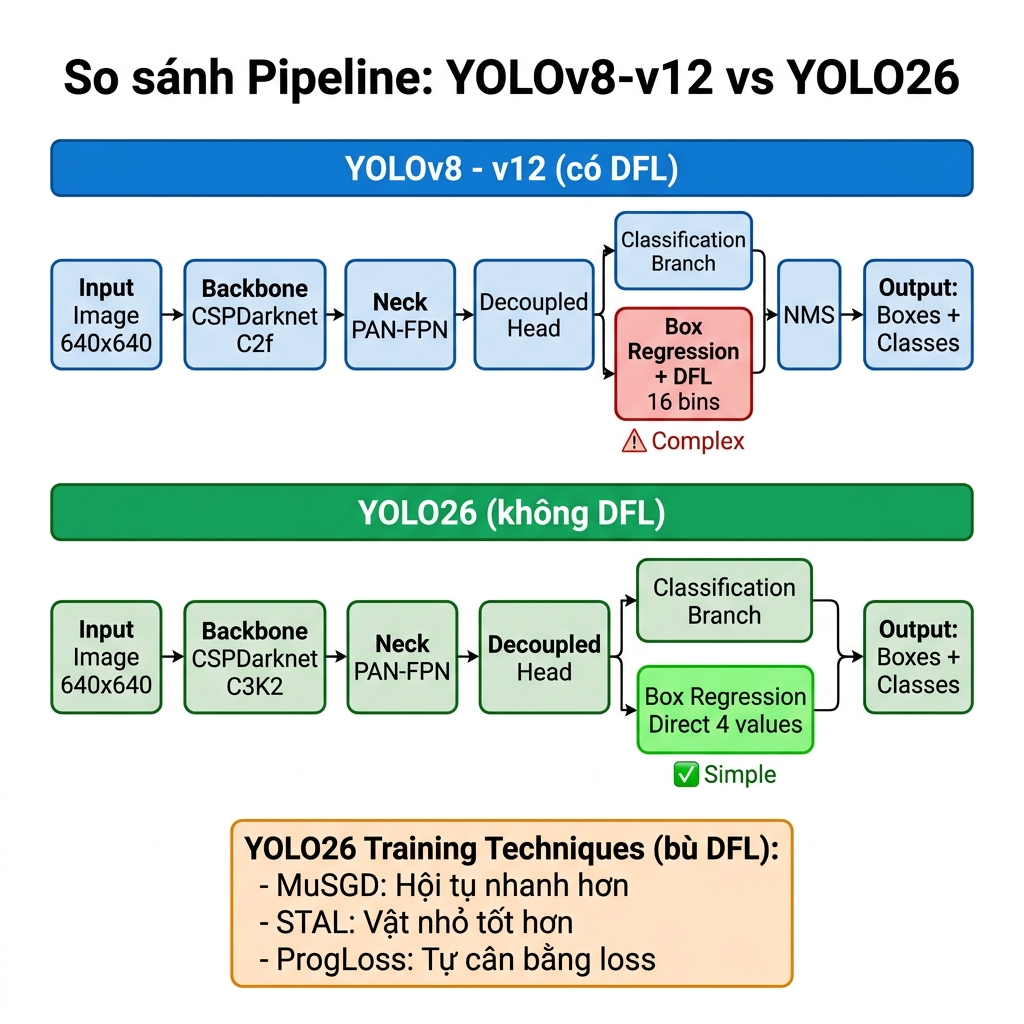
\includegraphics[width=\textwidth]{yolo26_pipeline.png}
\caption{So sánh pipeline: YOLOv8--v12 (có DFL) vs YOLO26 (không DFL). YOLO26 bù bằng 3 training techniques: MuSGD, STAL, ProgLoss.}
\end{figure}

% KẾT THÚC chuong6_yolo26
% ==========================================


% ==========================================
% BẮT ĐẦU chuong7_openvocab
% ==========================================
\chapter{BƯỚC NGOẶT OPEN-VOCABULARY}

\section{YOLO-World (2024) --- Tiên phong}
\textbf{Paper:} ``YOLO-World: Real-Time Open-Vocabulary Object Detection'' \cite{yoloworld}\\
\textbf{Tác giả:} Tencent AI Lab

\subsection{Ý tưởng cốt lõi}
Kết nối YOLO với \textbf{CLIP text embeddings} để detect bất kỳ vật nào chỉ bằng mô tả văn bản, không cần train lại. Dùng chiến lược \textbf{Prompt-then-Detect}: nạp text prompts 1 lần (offline), sau đó detect real-time.

\subsection{Kiến trúc}
\textbf{RepVL-PAN} (Re-parameterizable Vision-Language PAN) inject text features vào feature pyramid. Tách ``hiểu ngôn ngữ'' và ``detect'' thành 2 giai đoạn $\rightarrow$ inference nhanh.

\subsection{Nhận xét}

\textbf{Có gì mới?}
\begin{itemize}
    \item Lần đầu tiên YOLO có khả năng \textbf{open-vocabulary}: detect vật chưa từng train, chỉ cần gõ tên.
    \item YOLO-World-L đạt \textbf{35.4\% AP} (LVIS zero-shot) ở \textbf{52 FPS} (V100).
    \item Mở đường cho YOLOE và kỷ nguyên open-vocabulary detection.
\end{itemize}

\textbf{Hạn chế:}
\begin{itemize}
    \item Chỉ hỗ trợ \textbf{text prompt}, chưa hỗ trợ visual prompt (đưa ảnh mẫu).
    \item AP trên LVIS thấp hơn nhiều so với Grounding DINO (chậm hơn 10$\times$).
\end{itemize}

\textbf{Ví dụ:} YOLO truyền thống giống nhân viên bảo vệ chỉ nhận \textbf{80 khuôn mặt đã học}. YOLO-World giống bảo vệ có thể nhận diện bất kỳ ai --- chỉ cần bạn \textbf{mô tả bằng lời}: ``người mặc áo đỏ đội nón xanh''.

\section{YOLOE (2025) --- Real-Time Seeing Anything}
\textbf{Paper:} ``YOLOE: Real-Time Seeing Anything'' (ICCV 2025) \cite{yoloe}

\subsection{Ý tưởng cốt lõi}
Kết hợp \textbf{open-vocabulary + real-time} với 3 chế độ prompt: text (gõ tên), visual (đưa ảnh mẫu), và prompt-free (tự detect 1203 categories). Giải quyết hạn chế ``chỉ text prompt'' của YOLO-World.

\subsection{Kiến trúc}
3 module cho 3 chế độ: \textbf{RepRTA} (text prompt qua CLIP), \textbf{SAVPE} (visual prompt qua semantic + activation features), \textbf{LRPC} (prompt-free, pre-compute 1203 categories offline).

\subsection{Nhận xét}

\textbf{Có gì mới?}
\begin{itemize}
    \item \textbf{3 chế độ prompt}: Text (``tìm con chó''), Visual (đưa ảnh con chó mẫu), Prompt-Free (detect mọi thứ tự động).
    \item YOLOE-L đạt \textbf{27.1\% AP} (LVIS zero-shot) ở 48 FPS --- ngang Grounding DINO (27.4\%) nhưng \textbf{nhanh gấp 10$\times$}.
\end{itemize}

\textbf{Hạn chế:}
\begin{itemize}
    \item AP vẫn thấp hơn nhiều so với COCO closed-set (thang đo khác hoàn toàn).
    \item Visual prompt cần ảnh mẫu chất lượng tốt để hoạt động hiệu quả.
\end{itemize}

\textbf{Ví dụ:} Nếu YOLO-World giống bảo vệ nhận diện qua \textbf{lời mô tả}, thì YOLOE giống bảo vệ cao cấp hơn --- vừa nhận mô tả bằng lời, vừa nhận \textbf{ảnh mẫu}, hoặc thậm chí \textbf{tự phát hiện} mà không cần ai chỉ dẫn gì.

% KẾT THÚC chuong7_openvocab
% ==========================================


% ==========================================
% BẮT ĐẦU chuong8_bienthe
% ==========================================
\chapter{CÁC BIẾN THỂ YOLO}

\section{YOLOX (2021) --- Anchor-Free tiên phong}
\textbf{Tác giả:} Megvii \hfill \textbf{Giải thưởng:} 1st Place CVPR 2021 Streaming Perception

\subsection{Ý tưởng cốt lõi}
Chứng minh YOLO hoạt động tốt \textbf{không cần anchor boxes}, đồng thời giới thiệu \textbf{Decoupled Head} (tách cls/reg) và \textbf{SimOTA} (dynamic label assignment).

\subsection{Kiến trúc}
Backbone: Modified CSPDarknet. Head: \textbf{Decoupled} (2 branches riêng biệt cho classification và regression). Label assignment: \textbf{SimOTA} (simplified Optimal Transport Assignment).

\subsection{Nhận xét}

\textbf{Có gì mới?}
\begin{itemize}
    \item \textbf{3 kỹ thuật tiên phong} mà các đời YOLO sau đều adopt: Anchor-Free (v6, v8+), Decoupled Head (v6, v8, v11, v12), SimOTA $\rightarrow$ TAL (v8, v9, v10+).
    \item YOLOX-L đạt \textbf{50.0\% mAP} ở 69 FPS (V100). Nano variant chỉ \textbf{0.91M params}.
\end{itemize}

\textbf{Hạn chế:}
\begin{itemize}
    \item Không thuộc dòng chính YOLO (Redmon/Wang/Ultralytics) nên ecosystem nhỏ.
    \item SimOTA tốn computation hơn static assignment.
\end{itemize}

\textbf{Ví dụ:} YOLOX giống ``nhà phát minh'' --- tự mình không nổi tiếng bằng, nhưng 3 phát minh (Anchor-Free, Decoupled Head, SimOTA) đã được \textbf{toàn bộ thế hệ YOLO sau} áp dụng.

\section{PP-YOLOE (2022) --- Baidu Industrial}
\textbf{Tác giả:} Baidu \hfill \textbf{Framework:} PaddlePaddle

\subsection{Ý tưởng cốt lõi}
Giới thiệu \textbf{TAL (Task Alignment Learning)} --- alignment metric $t = s^\alpha \times u^\beta$ đảm bảo classification score cao $\leftrightarrow$ localization tốt. Tối ưu cho triển khai công nghiệp.

\subsection{Kiến trúc}
Backbone: CSPRepResNet. Neck: Custom PAN. Head: Efficient Task-Aligned Head với \textbf{TAL label assignment}. Anchor-free.

\subsection{Nhận xét}

\textbf{Có gì mới?}
\begin{itemize}
    \item \textbf{TAL}: Kỹ thuật gán nhãn thông minh nhất thời điểm đó --- được \textbf{YOLOv8, v9, v10+} adopt làm tiêu chuẩn.
    \item PP-YOLOE+-L đạt \textbf{53.3\% mAP} ở 78 FPS. Phổ biến trong công nghiệp Trung Quốc.
\end{itemize}

\textbf{Hạn chế:}
\begin{itemize}
    \item Chạy trên PaddlePaddle (Baidu) --- ecosystem nhỏ hơn PyTorch rất nhiều.
    \item Ít được cộng đồng quốc tế sử dụng ngoài Trung Quốc.
\end{itemize}

\textbf{Ví dụ:} TAL giống hệ thống chấm điểm ``2 tiêu chí'': vừa phải \textbf{nhận đúng người} (cls score cao), vừa phải \textbf{khoanh đúng vị trí} (IoU cao). Chỉ khi cả 2 đều tốt mới được coi là positive --- tránh tình trạng ``nhận đúng nhưng khoanh sai''.

\section{YOLO-NAS (2023) --- AI thiết kế AI}
\textbf{Tác giả:} Deci AI (Israel)

\subsection{Ý tưởng cốt lõi}
Dùng \textbf{AutoNAC} (Neural Architecture Search) để tự động khám phá $\sim 10^{14}$ kiến trúc và tìm tổ hợp tối ưu. Thiết kế sẵn cho quantization ngay từ đầu.

\subsection{Kiến trúc}
Backbone/Neck/Head đều do \textbf{AutoNAC tự thiết kế} --- không phải con người. Tối ưu đồng thời cho accuracy, latency, và quantization-friendliness.

\subsection{Nhận xét}

\textbf{Có gì mới?}
\begin{itemize}
    \item \textbf{NAS-designed}: Kiến trúc do AI tìm ra, không phải con người thiết kế thủ công.
    \item INT8 quantization chỉ mất \textbf{0.4--0.6\% mAP} (các model khác mất 1--2\%).
\end{itemize}

\textbf{Hạn chế:}
\begin{itemize}
    \item Weights không hoàn toàn open-source, cần license Deci AI cho một số tính năng.
    \item Kiến trúc NAS khó giải thích và tùy biến.
\end{itemize}

\textbf{Ví dụ:} Nếu YOLOv4--v12 giống xe do \textbf{kỹ sư con người} thiết kế (dựa trên kinh nghiệm và thí nghiệm), thì YOLO-NAS giống xe do \textbf{AI tự thiết kế} --- thử hàng nghìn tỉ tổ hợp rồi chọn ra xe tối ưu nhất.

% KẾT THÚC chuong8_bienthe
% ==========================================


% ==========================================
% BẮT ĐẦU chuong9_phahevakl
% ==========================================
\chapter{SƠ ĐỒ PHẢ HỆ YOLO VÀ KẾT LUẬN}

\section{Sơ đồ phả hệ YOLO (2015--2026)}

\begin{figure}[H]
\centering
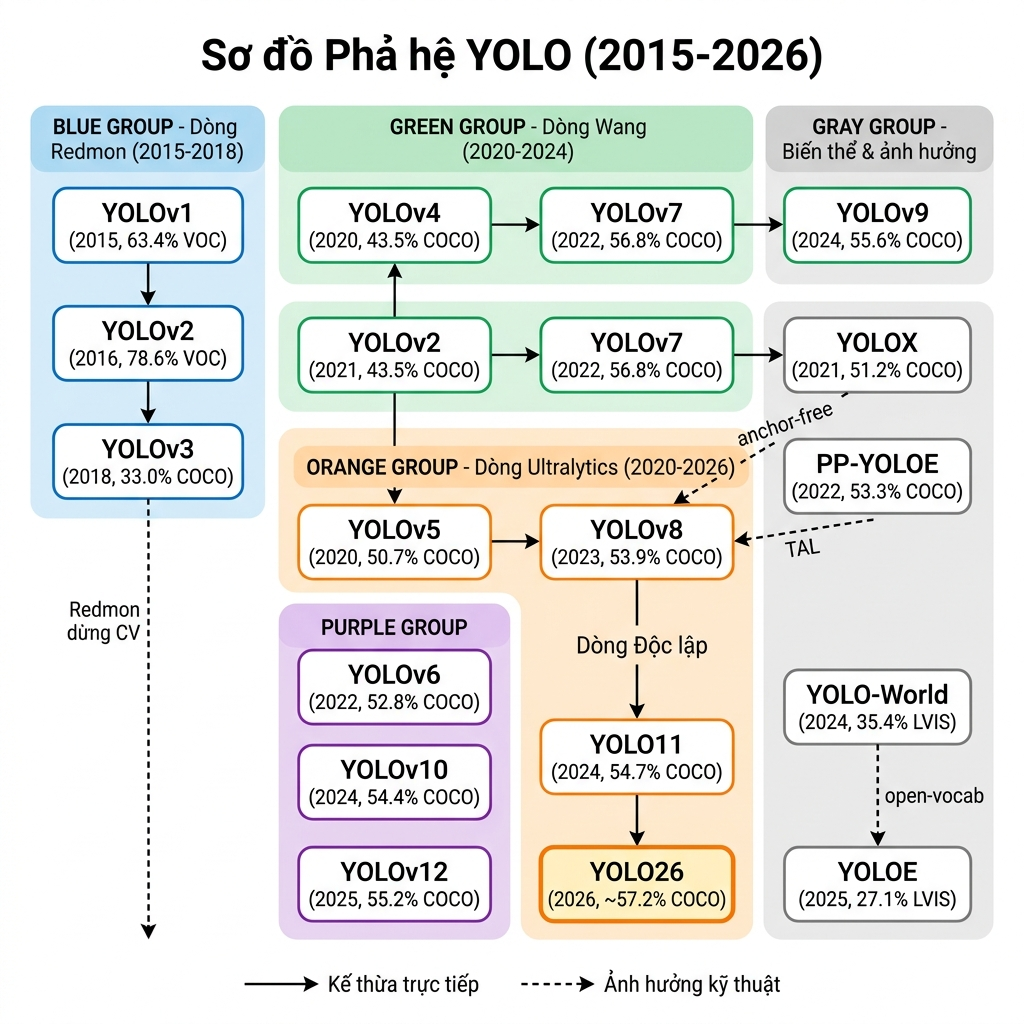
\includegraphics[width=\textwidth]{yolo_family_tree.png}
\caption{Sơ đồ phả hệ các phiên bản YOLO (2015--2026). Đường liền: kế thừa trực tiếp. Đường nét đứt: ảnh hưởng kỹ thuật.}
\end{figure}


\textit{Lưu ý: VOC mAP@50 (v1--v2) và COCO mAP@50:95 (v3+) là hai thang đo hoàn toàn khác nhau, không so sánh trực tiếp. LVIS zero-shot (YOLO-World, YOLOE) cũng là thang đo riêng.}

\section{Bảng tổng quan tất cả phiên bản}

\begin{table}[H]\centering
\caption{Tổng quan các phiên bản YOLO (2015--2026)}
\scriptsize
\begin{tabular}{lcccccccc}\toprule
\textbf{Version} & \textbf{Năm} & \textbf{mAP VOC@50} & \textbf{mAP COCO@50:95} & \textbf{FPS (GPU)} & \textbf{Params} & \textbf{Anchor} & \textbf{NMS} & \textbf{Paper}\\\midrule
v1 \cite{yolov1} & 2015 & 63.4\% & --- & 45 (Titan X) & $\sim$45M & Grid & Cần & Có \\
v2 \cite{yolov2} & 2016 & 78.6\% & --- & 67 (Titan X) & $\sim$50M & Có & Cần & Có \\
v3 \cite{yolov3} & 2018 & --- & 33.0\% & 20 (Titan X) & $\sim$62M & Có & Cần & Có \\
v4 \cite{yolov4} & 2020 & --- & 43.5\% & 65 (V100) & $\sim$64M & Có & Cần & Có \\
v5 \cite{yolov5} & 2020 & --- & 50.7\% & 98 (V100) & 86.7M & Có & Cần & Không \\
v6 \cite{yolov6} & 2022 & --- & 52.5\% & 116 (T4) & $\sim$58M & Không & Cần & Có \\
v7 \cite{yolov7} & 2022 & --- & 56.8\% & 36 (V100) & $\sim$71M & Có & Cần & Có \\
v8 \cite{yolov8} & 2023 & --- & 53.9\% & 83 (T4) & 68.2M & Không & Cần & Không \\
v9 \cite{yolov9} & 2024 & --- & 55.6\% & 57 (T4) & 58.1M & Không & Cần & Có \\
v10 \cite{yolov10} & 2024 & --- & 54.4\% & 96 (T4) & 29.5M & Không & \textbf{Không} & Có \\
YOLO11 \cite{yolo11} & 2024 & --- & 54.7\% & 79 (T4) & 56.9M & Không & Cần & Không \\
v12 \cite{yolov12} & 2025 & --- & 55.2\% & 51 (T4) & 59.1M & Không & Không & Có \\
YOLO26 \cite{yolo26} & 2026 & --- & $\sim$57.2\% & $\sim$102 (T4)$^*$ & $\sim$60M & Không & Không & Không \\
\bottomrule
\end{tabular}
\end{table}

\textit{$^*$ Ước tính. FPS = model size lớn nhất (v7-E6E, v5x, v8x...) trừ v1--v3 (model duy nhất). GPU ghi trong ngoặc. Lưu ý: Titan X, V100, T4 là 3 thế hệ GPU khác nhau --- FPS giữa chúng \textbf{không so sánh trực tiếp được}. v1--v2 dùng mAP VOC@50, v3+ dùng mAP COCO@50:95 --- hai thang đo hoàn toàn khác nhau.}

\section{Xếp hạng mAP COCO}

\begin{figure}[H]
\centering
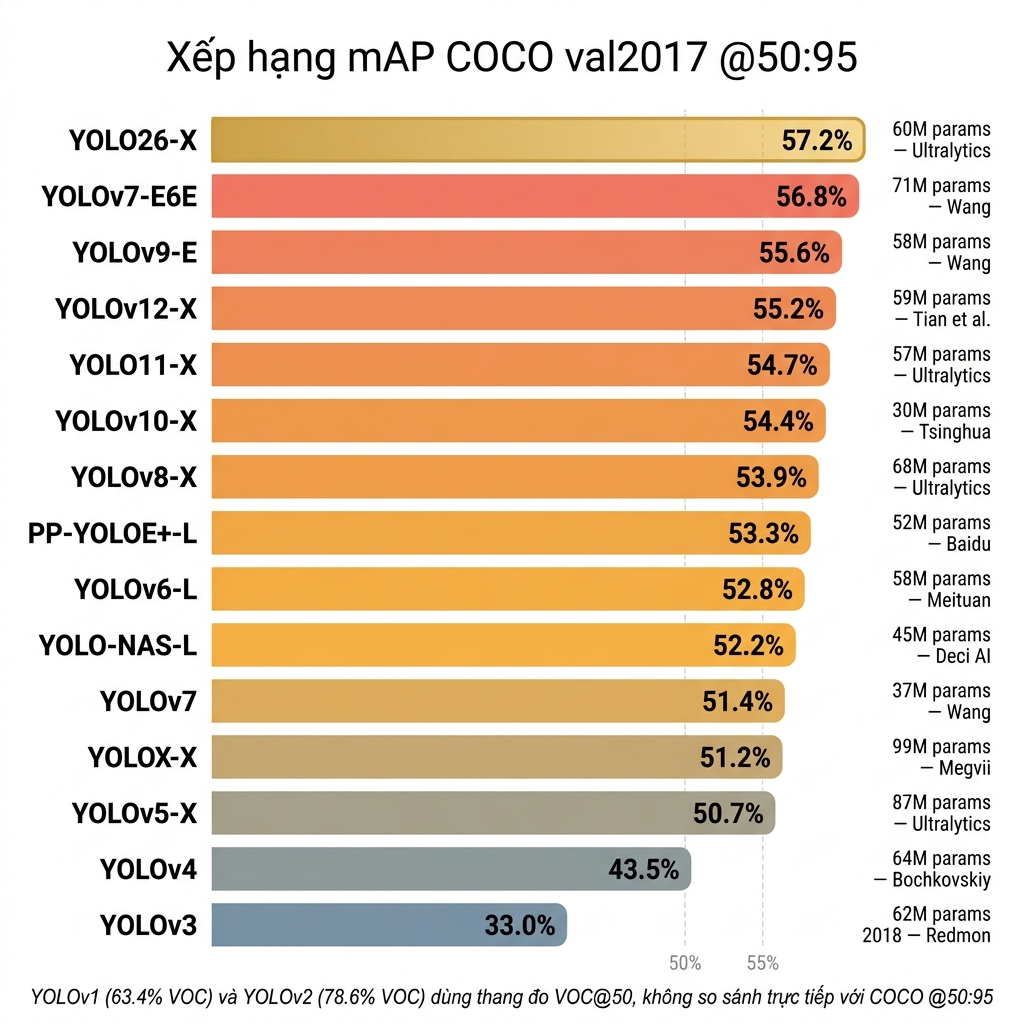
\includegraphics[width=0.9\textwidth]{pareto_chart.png}
\caption{Xếp hạng mAP COCO val2017 @50:95 --- tất cả phiên bản YOLO. Thanh trên cùng = model mạnh nhất hiện tại. YOLOv1--v2 dùng thang đo VOC@50 khác biệt.}
\end{figure}

\section{Tiến hóa công nghệ qua các phiên bản}

\begin{figure}[H]
\centering
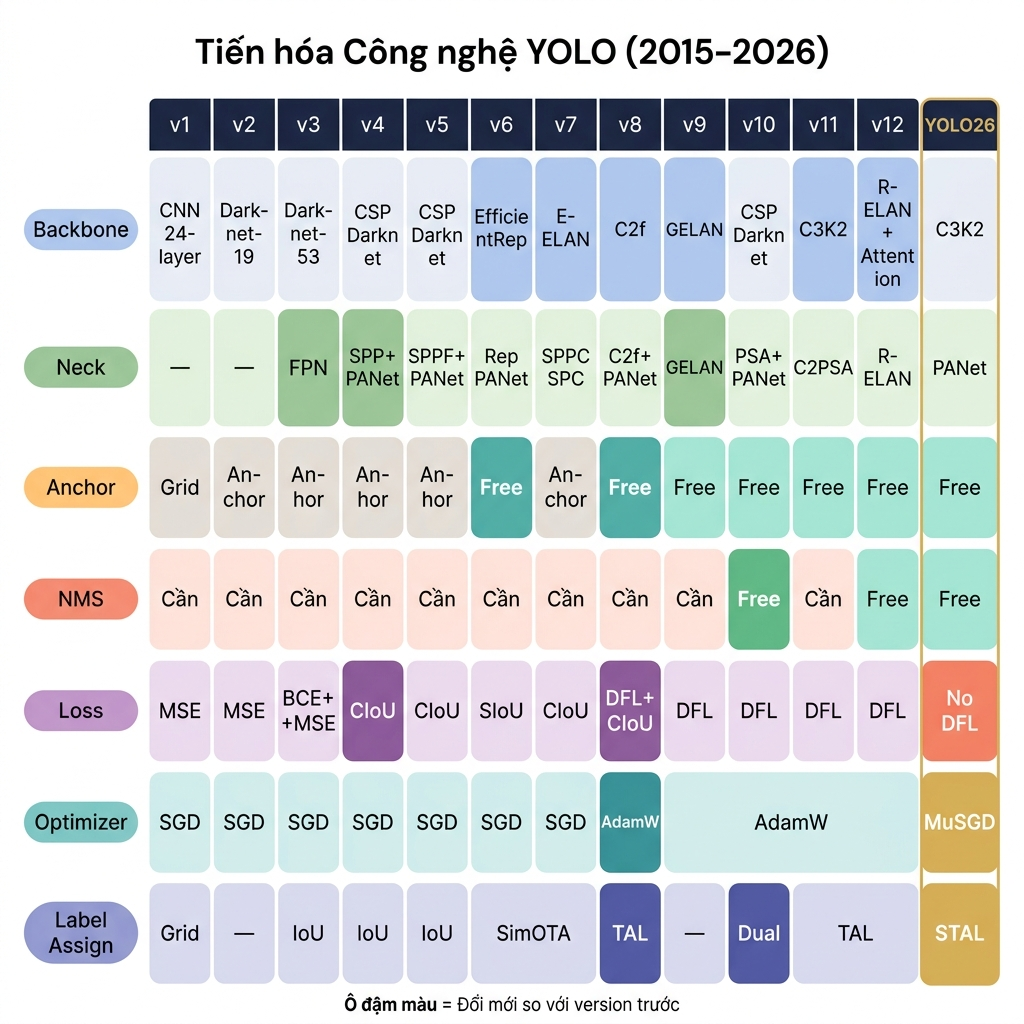
\includegraphics[width=\textwidth]{tech_evolution.png}
\caption{Tiến hóa công nghệ YOLO (2015--2026): Backbone, Anchor, NMS, Loss, Framework, Optimizer, và Label Assignment thay đổi qua từng phiên bản.}
\end{figure}

\section{Kết luận}

Qua 11 năm phát triển (2015--2026) và 14+ phiên bản, YOLO đã chứng minh: \textbf{không có ``model tốt nhất'' --- chỉ có ``model phù hợp nhất''}.

\textbf{Ba dòng phát triển song song} --- Redmon (v1--v3), Wang (v4,v7,v9), Ultralytics (v5,v8,v11,v26) --- cho thấy sức sống phi thường của triết lý ``You Only Look Once''.

\textbf{Các bước ngoặt quan trọng nhất:}
\begin{itemize}
    \item \textbf{YOLOv1} \cite{yolov1}: Chứng minh single-stage detection khả thi
    \item \textbf{YOLOv4} \cite{yolov4}: Hệ thống hóa BoF/BoS --- phương pháp luận nghiên cứu mẫu mực
    \item \textbf{YOLOv8} \cite{yolov8}: Anchor-free + 6 tasks --- dân chủ hóa object detection
    \item \textbf{YOLOv10} \cite{yolov10}: NMS-free --- giải quyết vấn đề tồn tại 9 năm
    \item \textbf{YOLOv12} \cite{yolov12}: Attention-centric --- mở kỷ nguyên mới
    \item \textbf{YOLO26} \cite{yolo26}: Edge-First + ``less is more'' --- bỏ DFL, bù bằng training techniques
\end{itemize}

\begin{quote}
\textit{``Chênh lệch 1--3\% mAP giữa các version trên COCO có thể không có ý nghĩa thống kê trên dataset thực tế. \textbf{Data chất lượng quan trọng hơn chọn model.}''}
\end{quote}

% KẾT THÚC chuong9_phahevakl
% ==========================================


\vspace{0.5cm}

\begin{thebibliography}{99}
\bibitem{yolov1} J. Redmon et al., ``You Only Look Once: Unified, Real-Time Object Detection,'' CVPR 2016. arXiv:1506.02640
\bibitem{yolov2} J. Redmon, A. Farhadi, ``YOLO9000: Better, Faster, Stronger,'' CVPR 2017. arXiv:1612.08242
\bibitem{yolov3} J. Redmon, A. Farhadi, ``YOLOv3: An Incremental Improvement,'' 2018. arXiv:1804.02767
\bibitem{yolov4} A. Bochkovskiy et al., ``YOLOv4: Optimal Speed and Accuracy of Object Detection,'' 2020. arXiv:2004.10934
\bibitem{yolov5} G. Jocher, ``YOLOv5,'' Ultralytics, 2020. github.com/ultralytics/yolov5
\bibitem{yolov6} C. Li et al., ``YOLOv6: A Single-Stage Object Detection Framework,'' 2022. arXiv:2209.02976
\bibitem{yolov7} C.-Y. Wang et al., ``YOLOv7: Trainable Bag-of-Freebies,'' CVPR 2023. arXiv:2207.02696
\bibitem{yolov8} G. Jocher, ``YOLOv8,'' Ultralytics, 2023. github.com/ultralytics/ultralytics
\bibitem{yolov9} C.-Y. Wang et al., ``YOLOv9: Learning What You Want to Learn Using PGI,'' 2024. arXiv:2402.13616
\bibitem{yolov10} A. Wang et al., ``YOLOv10: Real-Time End-to-End Object Detection,'' 2024. arXiv:2405.14458
\bibitem{yolo11} G. Jocher, ``YOLO11,'' Ultralytics, 2024. github.com/ultralytics/ultralytics
\bibitem{yolov12} Y. Tian et al., ``YOLOv12: Attention-Centric Real-Time Object Detectors,'' 2025. arXiv:2502.12524
\bibitem{yoloe} ``YOLOE: Real-Time Seeing Anything,'' ICCV 2025. arXiv:2503.07465
\bibitem{yolo26} G. Jocher, ``YOLO26,'' Ultralytics, 2026. github.com/ultralytics/ultralytics
\bibitem{yolox} Z. Ge et al., ``YOLOX: Exceeding YOLO Series in 2021,'' 2021. arXiv:2107.08430
\bibitem{ppyoloe} S. Xu et al., ``PP-YOLOE: An Evolved Version of YOLO,'' 2022. arXiv:2203.16250
\bibitem{yolonas} ``YOLO-NAS,'' Deci AI, 2023. github.com/Deci-AI/super-gradients
\bibitem{yoloworld} T. Cheng et al., ``YOLO-World: Real-Time Open-Vocabulary Object Detection,'' 2024. arXiv:2401.17270
\end{thebibliography}

% BẮT ĐẦU phuluc_thuatngu
% ==========================================
\chapter*{PHỤ LỤC: BẢNG THUẬT NGỮ}
\addcontentsline{toc}{chapter}{Phụ lục: Bảng thuật ngữ}

Dưới đây là các thuật ngữ kỹ thuật thường gặp trong lĩnh vực YOLO và Object Detection, sắp xếp theo nhóm chủ đề.

\section*{Kiến trúc mạng (Architecture)}

\begin{longtable}{p{3.5cm}p{12cm}}
\toprule
\textbf{Thuật ngữ} & \textbf{Giải thích} \\
\midrule
\endfirsthead
\toprule
\textbf{Thuật ngữ} & \textbf{Giải thích} \\
\midrule
\endhead

\textbf{Backbone} & Phần ``xương sống'' của model, trích xuất features từ ảnh đầu vào. Ví dụ: Darknet, CSPDarknet, ResNet, EfficientNet. \\
\midrule
\textbf{Neck} & Kết nối Backbone và Head, kết hợp features ở nhiều scales. Ví dụ: FPN, PAN, BiFPN. \\
\midrule
\textbf{Head} & Phần cuối cùng, dự đoán bounding boxes và class probabilities. Có 2 loại: coupled (chung) và decoupled (tách riêng cls/reg). \\
\midrule
\textbf{CNN} & Convolutional Neural Network --- mạng neural dùng phép tích chập (convolution) để trích xuất features từ ảnh. Mỗi layer học nhận diện patterns (cạnh, góc, hình dạng). \\
\midrule
\textbf{Convolution} & Phép tính trượt 1 bộ lọc (kernel) qua ảnh, tạo feature map. Kernel $3\times3$ nhìn vùng $3\times3$ pixels. \\
\midrule
\textbf{Depthwise Conv} & Convolution áp dụng riêng cho từng channel (thay vì tất cả channels cùng lúc) --- giảm computation đáng kể. \\
\midrule
\textbf{Residual Connection} & Đường tắt (shortcut) nối input trực tiếp đến output: $y = F(x) + x$. Giải quyết vanishing gradient khi mạng rất sâu (ResNet). \\
\midrule
\textbf{CSP} & Cross Stage Partial --- chia features thành 2 phần: 1 phần qua processing, 1 phần bypass $\rightarrow$ giảm 20\% computation. \\
\midrule
\textbf{FPN} & Feature Pyramid Network --- kết hợp features từ nhiều scales (top-down pathway) để detect vật ở mọi kích thước. \\
\midrule
\textbf{PAN / PANet} & Path Aggregation Network --- thêm bottom-up pathway vào FPN $\rightarrow$ localization signals mạnh hơn. \\
\midrule
\textbf{SPP / SPPF} & Spatial Pyramid Pooling --- MaxPool nhiều kích thước $\rightarrow$ tăng receptive field. SPPF: phiên bản nhanh hơn (nối tiếp thay song song). \\
\midrule
\textbf{Re-parameterization} & Kỹ thuật training multi-branch, inference single-branch. Gộp nhiều Conv thành 1 Conv duy nhất bằng phép cộng ma trận. \\
\midrule
\textbf{Attention} & Cơ chế cho model ``tập trung'' vào vùng quan trọng. Self-attention so sánh mọi vị trí với nhau (global receptive field). \\
\midrule
\textbf{FlashAttention} & Thuật toán tính attention tối ưu memory --- giảm memory footprint đáng kể, cho phép dùng attention trên feature maps lớn. \\
\bottomrule
\end{longtable}

\section*{Kỹ thuật Detection}

\begin{longtable}{p{3.5cm}p{12cm}}
\toprule
\textbf{Thuật ngữ} & \textbf{Giải thích} \\
\midrule
\endfirsthead
\toprule
\textbf{Thuật ngữ} & \textbf{Giải thích} \\
\midrule
\endhead

\textbf{Bounding Box} & Hình chữ nhật bao quanh vật thể, xác định vị trí (x, y, width, height). \\
\midrule
\textbf{Anchor Box} & Hộp mẫu (template) được định nghĩa trước. Model dự đoán offsets so với anchor thay vì tọa độ tuyệt đối. v2--v7 dùng anchor, v8+ bỏ anchor. \\
\midrule
\textbf{Anchor-free} & Không dùng anchor. Dự đoán trực tiếp center point + 4 distances (khoảng cách từ tâm đến 4 cạnh). Đơn giản hơn anchor-based. \\
\midrule
\textbf{NMS} & Non-Maximum Suppression --- thuật toán loại bỏ bounding boxes trùng lặp. Giữ box confidence cao nhất, bỏ các boxes có IoU lớn. \\
\midrule
\textbf{NMS-free} & Không cần NMS --- model tự output 1 box/vật. Từ v10 trở đi. Dùng dual assignment (o2m + o2o). \\
\midrule
\textbf{Decoupled Head} & Tách classification và regression thành 2 branches riêng biệt. YOLOX giới thiệu, v6, v8+ adopt. \\
\midrule
\textbf{Label Assignment} & Chiến lược gán prediction cho ground truth khi training. SimOTA (động), TAL (task-aligned), STAL (small-target-aware). \\
\midrule
\textbf{End-to-End} & Pipeline từ input đến output không cần bước xử lý thủ công trung gian (ví dụ: không cần NMS). \\
\midrule
\textbf{Multi-scale} & Dự đoán ở nhiều kích thước (scales). YOLOv3+: 3 scales (lớn/trung/nhỏ) để detect vật ở mọi kích thước. \\
\midrule
\textbf{One-stage / Two-stage} & One-stage: 1 lần forward pass ra kết quả (YOLO). Two-stage: region proposal + classification (Faster R-CNN). \\
\bottomrule
\end{longtable}

\section*{Metrics (Chỉ số đánh giá)}

\begin{longtable}{p{3.5cm}p{12cm}}
\toprule
\textbf{Thuật ngữ} & \textbf{Giải thích} \\
\midrule
\endfirsthead
\toprule
\textbf{Thuật ngữ} & \textbf{Giải thích} \\
\midrule
\endhead

\textbf{IoU} & Intersection over Union --- đo mức trùng lặp giữa predicted box và ground truth. $IoU = \frac{Giao}{Hop}$. Từ 0 (không trùng) đến 1 (trùng hoàn hảo). \\
\midrule
\textbf{mAP} & mean Average Precision --- trung bình AP trên tất cả classes. Metric chính đánh giá detection. \\
\midrule
\textbf{mAP@50} & AP ở ngưỡng IoU $\geq$ 0.5. Dùng trên VOC. \\
\midrule
\textbf{mAP@50:95} & Trung bình AP ở IoU từ 0.5 đến 0.95 (bước 0.05). Metric chính trên COCO --- khắt khe hơn mAP@50. \\
\midrule
\textbf{FPS} & Frames Per Second --- số ảnh xử lý mỗi giây. $\geq$30 FPS = real-time. \\
\midrule
\textbf{Params} & Số lượng tham số của model. Ví dụ: 3.2M = 3.2 triệu tham số. Ít params = model nhẹ. \\
\midrule
\textbf{FLOPs / GFLOPs} & Floating Point Operations --- số phép tính cần thực hiện. Đo computational cost. 1 GFLOPs = 1 tỷ phép tính. \\
\midrule
\textbf{Latency} & Thời gian xử lý 1 ảnh (ms). Khác FPS vì bao gồm cả pre/post-processing. \\
\bottomrule
\end{longtable}

\section*{Training (Huấn luyện)}

\begin{longtable}{p{3.5cm}p{12cm}}
\toprule
\textbf{Thuật ngữ} & \textbf{Giải thích} \\
\midrule
\endfirsthead
\toprule
\textbf{Thuật ngữ} & \textbf{Giải thích} \\
\midrule
\endhead

\textbf{Batch Normalization} & Chuẩn hóa output mỗi layer theo mini-batch $\rightarrow$ training ổn định hơn, nhanh hội tụ hơn. YOLOv2 thêm BN: +2\% mAP. \\
\midrule
\textbf{Mosaic} & Data augmentation ghép 4 ảnh thành 1 $\rightarrow$ model thấy nhiều context, giảm batch size cần thiết. YOLOv4 giới thiệu. \\
\midrule
\textbf{CutMix} & Cắt 1 vùng từ ảnh A dán vào ảnh B, mix labels theo tỷ lệ diện tích. \\
\midrule
\textbf{Augmentation} & Biến đổi ảnh khi training (xoay, lật, zoom, đổi màu...) để model tổng quát hơn. \\
\midrule
\textbf{Transfer Learning} & Dùng model đã train trên dataset lớn (ImageNet) $\rightarrow$ fine-tune trên dataset nhỏ của mình. Tiết kiệm thời gian, ít data hơn. \\
\midrule
\textbf{Quantization} & Giảm precision từ FP32 (32-bit) xuống INT8 (8-bit) $\rightarrow$ model nhẹ hơn 4$\times$, nhanh hơn, nhưng có thể mất accuracy. \\
\midrule
\textbf{PTQ} & Post-Training Quantization --- quantize sau khi train xong. Nhanh nhưng mất accuracy. \\
\midrule
\textbf{QAT} & Quantization-Aware Training --- train lại với simulated quantization $\rightarrow$ giữ accuracy tốt hơn PTQ. \\
\midrule
\textbf{BoF / BoS} & Bag of Freebies (tăng training cost, không tăng inference) / Bag of Specials (tăng nhẹ inference cost). YOLOv4 hệ thống hóa. \\
\bottomrule
\end{longtable}

\section*{Loss Functions (Hàm mất mát)}

\begin{longtable}{p{3.5cm}p{12cm}}
\toprule
\textbf{Thuật ngữ} & \textbf{Giải thích} \\
\midrule
\endfirsthead
\toprule
\textbf{Thuật ngữ} & \textbf{Giải thích} \\
\midrule
\endhead

\textbf{MSE / SSE} & Mean/Sum Squared Error --- đo sai số bình phương. v1--v3 dùng cho box coordinates. \\
\midrule
\textbf{IoU Loss} & $\mathcal{L} = 1 - IoU$. Trực tiếp tối ưu IoU thay vì tọa độ riêng lẻ. \\
\midrule
\textbf{GIoU} & Generalized IoU --- xét cả vùng bao ngoài 2 boxes. Giải quyết trường hợp 2 box không giao nhau (IoU = 0 nhưng GIoU $\neq$ 0). \\
\midrule
\textbf{CIoU} & Complete IoU --- thêm khoảng cách tâm + aspect ratio vào GIoU. $\mathcal{L}_{CIoU} = 1 - IoU + \frac{\rho^2}{c^2} + \alpha v$. YOLOv4+ dùng. \\
\midrule
\textbf{DFL} & Distribution Focal Loss --- dự đoán phân phối xác suất cho box coordinates (16 bins) thay vì 1 giá trị. v8--v12 dùng, YOLO26 bỏ. \\
\midrule
\textbf{BCE} & Binary Cross-Entropy --- loss cho classification. v3+ dùng BCE thay Softmax để hỗ trợ multi-label. \\
\bottomrule
\end{longtable}

\section*{Deployment (Triển khai)}

\begin{longtable}{p{3.5cm}p{12cm}}
\toprule
\textbf{Thuật ngữ} & \textbf{Giải thích} \\
\midrule
\endfirsthead
\toprule
\textbf{Thuật ngữ} & \textbf{Giải thích} \\
\midrule
\endhead

\textbf{ONNX} & Open Neural Network Exchange --- format chuẩn để export model, chạy được trên nhiều frameworks/hardware. \\
\midrule
\textbf{TensorRT} & NVIDIA SDK tối ưu inference trên GPU NVIDIA. Tăng 2--5$\times$ speed so với PyTorch. \\
\midrule
\textbf{Edge deployment} & Triển khai model trên thiết bị nhỏ (mobile, camera, drone) thay vì server lớn. Cần model nhẹ, ít computation. \\
\midrule
\textbf{FP16 / FP32} & Float 16-bit / 32-bit precision. FP16 nhanh hơn, ít memory hơn, gần như không mất accuracy. \\
\midrule
\textbf{INT8} & Integer 8-bit. Nhẹ hơn FP32 gấp 4$\times$ nhưng có thể mất 0.5--2\% accuracy. \\
\bottomrule
\end{longtable}

% KẾT THÚC phuluc_thuatngu
% ==========================================


\end{document}

